% Options for packages loaded elsewhere
\PassOptionsToPackage{unicode}{hyperref}
\PassOptionsToPackage{hyphens}{url}
%
\documentclass[
]{book}
\title{Writing games with Python and PsychoPy}
\author{Alexander (Sasha) Pastukhov}
\date{2021-10-06}

\usepackage{amsmath,amssymb}
\usepackage{lmodern}
\usepackage{iftex}
\ifPDFTeX
  \usepackage[T1]{fontenc}
  \usepackage[utf8]{inputenc}
  \usepackage{textcomp} % provide euro and other symbols
\else % if luatex or xetex
  \usepackage{unicode-math}
  \defaultfontfeatures{Scale=MatchLowercase}
  \defaultfontfeatures[\rmfamily]{Ligatures=TeX,Scale=1}
\fi
% Use upquote if available, for straight quotes in verbatim environments
\IfFileExists{upquote.sty}{\usepackage{upquote}}{}
\IfFileExists{microtype.sty}{% use microtype if available
  \usepackage[]{microtype}
  \UseMicrotypeSet[protrusion]{basicmath} % disable protrusion for tt fonts
}{}
\makeatletter
\@ifundefined{KOMAClassName}{% if non-KOMA class
  \IfFileExists{parskip.sty}{%
    \usepackage{parskip}
  }{% else
    \setlength{\parindent}{0pt}
    \setlength{\parskip}{6pt plus 2pt minus 1pt}}
}{% if KOMA class
  \KOMAoptions{parskip=half}}
\makeatother
\usepackage{xcolor}
\IfFileExists{xurl.sty}{\usepackage{xurl}}{} % add URL line breaks if available
\IfFileExists{bookmark.sty}{\usepackage{bookmark}}{\usepackage{hyperref}}
\hypersetup{
  pdftitle={Writing games with Python and PsychoPy},
  pdfauthor={Alexander (Sasha) Pastukhov},
  hidelinks,
  pdfcreator={LaTeX via pandoc}}
\urlstyle{same} % disable monospaced font for URLs
\usepackage{color}
\usepackage{fancyvrb}
\newcommand{\VerbBar}{|}
\newcommand{\VERB}{\Verb[commandchars=\\\{\}]}
\DefineVerbatimEnvironment{Highlighting}{Verbatim}{commandchars=\\\{\}}
% Add ',fontsize=\small' for more characters per line
\usepackage{framed}
\definecolor{shadecolor}{RGB}{248,248,248}
\newenvironment{Shaded}{\begin{snugshade}}{\end{snugshade}}
\newcommand{\AlertTok}[1]{\textcolor[rgb]{0.94,0.16,0.16}{#1}}
\newcommand{\AnnotationTok}[1]{\textcolor[rgb]{0.56,0.35,0.01}{\textbf{\textit{#1}}}}
\newcommand{\AttributeTok}[1]{\textcolor[rgb]{0.77,0.63,0.00}{#1}}
\newcommand{\BaseNTok}[1]{\textcolor[rgb]{0.00,0.00,0.81}{#1}}
\newcommand{\BuiltInTok}[1]{#1}
\newcommand{\CharTok}[1]{\textcolor[rgb]{0.31,0.60,0.02}{#1}}
\newcommand{\CommentTok}[1]{\textcolor[rgb]{0.56,0.35,0.01}{\textit{#1}}}
\newcommand{\CommentVarTok}[1]{\textcolor[rgb]{0.56,0.35,0.01}{\textbf{\textit{#1}}}}
\newcommand{\ConstantTok}[1]{\textcolor[rgb]{0.00,0.00,0.00}{#1}}
\newcommand{\ControlFlowTok}[1]{\textcolor[rgb]{0.13,0.29,0.53}{\textbf{#1}}}
\newcommand{\DataTypeTok}[1]{\textcolor[rgb]{0.13,0.29,0.53}{#1}}
\newcommand{\DecValTok}[1]{\textcolor[rgb]{0.00,0.00,0.81}{#1}}
\newcommand{\DocumentationTok}[1]{\textcolor[rgb]{0.56,0.35,0.01}{\textbf{\textit{#1}}}}
\newcommand{\ErrorTok}[1]{\textcolor[rgb]{0.64,0.00,0.00}{\textbf{#1}}}
\newcommand{\ExtensionTok}[1]{#1}
\newcommand{\FloatTok}[1]{\textcolor[rgb]{0.00,0.00,0.81}{#1}}
\newcommand{\FunctionTok}[1]{\textcolor[rgb]{0.00,0.00,0.00}{#1}}
\newcommand{\ImportTok}[1]{#1}
\newcommand{\InformationTok}[1]{\textcolor[rgb]{0.56,0.35,0.01}{\textbf{\textit{#1}}}}
\newcommand{\KeywordTok}[1]{\textcolor[rgb]{0.13,0.29,0.53}{\textbf{#1}}}
\newcommand{\NormalTok}[1]{#1}
\newcommand{\OperatorTok}[1]{\textcolor[rgb]{0.81,0.36,0.00}{\textbf{#1}}}
\newcommand{\OtherTok}[1]{\textcolor[rgb]{0.56,0.35,0.01}{#1}}
\newcommand{\PreprocessorTok}[1]{\textcolor[rgb]{0.56,0.35,0.01}{\textit{#1}}}
\newcommand{\RegionMarkerTok}[1]{#1}
\newcommand{\SpecialCharTok}[1]{\textcolor[rgb]{0.00,0.00,0.00}{#1}}
\newcommand{\SpecialStringTok}[1]{\textcolor[rgb]{0.31,0.60,0.02}{#1}}
\newcommand{\StringTok}[1]{\textcolor[rgb]{0.31,0.60,0.02}{#1}}
\newcommand{\VariableTok}[1]{\textcolor[rgb]{0.00,0.00,0.00}{#1}}
\newcommand{\VerbatimStringTok}[1]{\textcolor[rgb]{0.31,0.60,0.02}{#1}}
\newcommand{\WarningTok}[1]{\textcolor[rgb]{0.56,0.35,0.01}{\textbf{\textit{#1}}}}
\usepackage{longtable,booktabs,array}
\usepackage{calc} % for calculating minipage widths
% Correct order of tables after \paragraph or \subparagraph
\usepackage{etoolbox}
\makeatletter
\patchcmd\longtable{\par}{\if@noskipsec\mbox{}\fi\par}{}{}
\makeatother
% Allow footnotes in longtable head/foot
\IfFileExists{footnotehyper.sty}{\usepackage{footnotehyper}}{\usepackage{footnote}}
\makesavenoteenv{longtable}
\usepackage{graphicx}
\makeatletter
\def\maxwidth{\ifdim\Gin@nat@width>\linewidth\linewidth\else\Gin@nat@width\fi}
\def\maxheight{\ifdim\Gin@nat@height>\textheight\textheight\else\Gin@nat@height\fi}
\makeatother
% Scale images if necessary, so that they will not overflow the page
% margins by default, and it is still possible to overwrite the defaults
% using explicit options in \includegraphics[width, height, ...]{}
\setkeys{Gin}{width=\maxwidth,height=\maxheight,keepaspectratio}
% Set default figure placement to htbp
\makeatletter
\def\fps@figure{htbp}
\makeatother
\setlength{\emergencystretch}{3em} % prevent overfull lines
\providecommand{\tightlist}{%
  \setlength{\itemsep}{0pt}\setlength{\parskip}{0pt}}
\setcounter{secnumdepth}{5}
\usepackage{booktabs}
\ifLuaTeX
  \usepackage{selnolig}  % disable illegal ligatures
\fi
\usepackage[]{natbib}
\bibliographystyle{apalike}

\begin{document}
\maketitle

{
\setcounter{tocdepth}{1}
\tableofcontents
}
\hypertarget{intro}{%
\chapter{Introduction}\label{intro}}

This book will teach you programming. Hopefully, it will do so in a fun way because if there is something more satisfying than playing a video game then it is creating one. Although it is written for the course called \emph{``Python for social and experimental psychology''}, my main aim is not to teach you Python per se. Python is a fantastic tool (more on this later) but it is just one of many programming languages that exist. My ultimate goal is to help you to develop general programming skills, which do not depend on a specific-programming language, and make sure that you form good habits that will make your code clear, easy to read, and easy to maintain. That last part is crucial. Programming is not about writing code that works. That, obviously, must be true but it is only the minimal requirement. Programming is about writing a clear and easy-to-read code that others and, even more importantly, you-two-weeks later can understand.

\hypertarget{prerequisites}{%
\section{Prerequisites}\label{prerequisites}}

The material assumes no foreknowledge of Python or programming from the reader. Its purpose is to gradually build up your knowledge and allow you to create more and more complex games.

\hypertarget{why-games}{%
\section{Why games?}\label{why-games}}

The actual purpose of this course is to teach psychology and social studies students in how to program \emph{experiments}. That is what the real research is about. However, there is little practical difference between the two. The basic ingredients are the same and, arguably, experiments are just boring games. And, be assured, if you can program a game, you can certainly program an experiment.

\hypertarget{why-should-a-psychologist-learn-programming}{%
\section{Why should a psychologist learn programming?}\label{why-should-a-psychologist-learn-programming}}

Why should a psychologist, who is interested in people, learn how to program computers? The most obvious questions is that is this a useful skill. Being able to program gives you freedom to create an experiment that answers your research question, not an experiment that can be implemented given constraints of your software.

More importantly, at least from my point of view, is that learning programming changes the way you think in general. People are smart but computers are dumb. When you explain your experiment or travel plans to somebody, you can be fairly vague, make a minor mistake, even skip certain parts. People are smart so they will fill the missing information in with their knowledge, spot and correct a mistake, ask you for more information, and can improvise on their own once they encounter something that you have not covered. Computers are dumb, so you must be precise, you cannot have gray areas, you cannot leave anything to ``it will figure it out once it happens'' (it won't). My personal experience, corroborated by psychologists who learned programming, is that it makes you realize just how vague and imprecise people can be without realizing it. Programming forces you to be precise and thorough, to plan ahead for any eventuality there might be. And this is a very useful skill by itself as it can be applied to any activity that requires planning be that an experimental design or travel arrangements.

\hypertarget{why-python}{%
\section{Why Python?}\label{why-python}}

There are many ways to create an experiment for psychological research. You can use drag-and-drop systems either commercial like \href{https://www.neurobs.com/}{Presentation}, \href{https://www.sr-research.com/experiment-builder/}{Experiment Builder} or free like \href{https://psychopy.org/builder}{PsychoPy Bulder interface}. They have a much shallower learning curve, so you can start creating and running your experiments faster. However, the simplicity of their use has a price: They are fairly limited in which stimuli you can use and how you can control the presentation schedule, conditions, feedback, etc. Typically, they allow you to extend them by programming the desired behavior but you do need to know how to program to do this (knowing Python supercharges your PsychoPy experiments). Thus, I think that while these systems, in particular \href{https://psychopy.org/}{PsychoPy}, are great tools to quickly bang a simple experiment together, they are most useful if you understand how they create the underlying code and how you would program it yourself. Then, you will not be limited by the software, as you know you can program something the default drag-and-drop won't allow. At the same time, you can always opt in, if drag-and-drop is sufficient but faster. At the end, it is about having options and creative freedom to program an experiment that will answer your research question, not an experiment that your software allows you to program.

We will learn programming in Python, which is a great language that combines simple and clear syntax with power and ability to tackle almost any problem. In this seminar, we will concentrate on desktop experiments but you can use it for online experiments (\href{https://otree.readthedocs.io/en/latest/}{oTree} and \href{https://psychopy.org/}{PsychoPy}), scientific programming (\href{https://numpy.org/}{NumPy} and \href{https://www.scipy.org/}{SciPy}), data analysis (\href{https://pandas.pydata.org/}{pandas}), machine learning (\href{https://keras.io/}{keras}), website programming (\href{https://www.djangoproject.com/}{django}), computer vision (\href{https://opencv.org/}{OpenCV}), etc. Thus, Python is one of the most versatile programming tools that you can use for all stages of your research or work. And, Python is free, so you do not need to worry whether you or your future employer will be able to afford license fees (a very real problem, if you use Matlab).

\hypertarget{seminar-specific-information}{%
\section{Seminar-specific information}\label{seminar-specific-information}}

This is a material for \emph{Python for social and experimental psychology} seminar as taught by me at the University of Bamberg. Each chapter covers a single game, introducing necessary ideas and is accompanied by exercises that you need to complete and submit. To pass the seminar, you will need to complete all assignments, i.e., write all the games. You do not need to complete or provide correct solutions for \emph{all} the exercises to pass the course and information on how the points for exercises will be converted to an actual grade (if you need one) or ``pass'' will be available during the seminar.

The material is structured, so that each chapter or chapter section correspond to a single meeting. However, we are all different, so work at your own pace. You can read the material and submit assignments independently. I will provide detailed feedback for each assignment and you will have an opportunity to address issues and resubmit again with no loss of points. Note that my feedback will cover not only the actual problems with the code but the way you implemented the solution and how nice-looking your code is. Remember, our task is not just to learn how to program a working game but how to write a nice clear easy-to-read-and-maintain code\footnote{Good habits! Form good habits! Thank you for reading this subliminal message.}.

Very important: Do not hesitate to ask questions. If I feel that you missed the information in the material, I will point you to the exact location. If you are confused, I'll gently prod you with questions so that you will solve your own problem. If you need more information, I'll supply it. If you simply want to know more, ask and I'll explain why things are the way they are or suggest what to read. If I feel that you should be able to solve the issue without my help, I'll tell you so (although, I would still probably ask a few hinting questions).

\hypertarget{about-the-material}{%
\section{About the material}\label{about-the-material}}

This material is \textbf{free to use} and is licensed under the \href{https://creativecommons.org/licenses/by-nc-nd/4.0/}{Creative Commons Attribution-NonCommercial-NoDerivatives V4.0 International License}.

\hypertarget{software}{%
\chapter{Software}\label{software}}

For this book and seminar, we will need to install

\begin{itemize}
\tightlist
\item
  PsychoPy that comes bundled with Python.
\item
  IDE of your choice. My instructions will be for Visual Studio Code, which has a very good Python support.
\item
  Jupyter Notebook for trying out small snippets of code.
\end{itemize}

I will not give detailed instructions on how to install the necessary software but rather point you to official manuals. This makes this text more future-proof as specific details might easily change\footnote{If you are part of the seminar, ask me whenever you have problems or are unsure about how to proceeed}.

\hypertarget{install-psychopy}{%
\section{PsychoPy}\label{install-psychopy}}

Download and install \href{https://www.psychopy.org/download.html}{Standalone PsychoPy} version. Use whatever the latest (and greatest) PsychoPy version is suggested to you (PsychoPy 2021.2.3 using Python3.6 as of time of writing) and follow instructions.

Note that you can also install PsychoPy as a anaconda package or install an official Python distribution and add PsychoPy via pip. However, I find the standalone easier to use as it has all necessary additional libraries. Plus, it has additional tools for GUI-based experiment programming and integration with \url{Pavlovia.org}.

\hypertarget{install-vs-code}{%
\section{VS Code}\label{install-vs-code}}

\href{https://code.visualstudio.com/}{Visual Studio Code} is a free lightweight open-source editor with strong support for Python. Download the installer for your platform and follow the instructions.

Next, follow \href{https://code.visualstudio.com/docs/python/python-tutorial}{Getting Started with Python in VS Code} tutorial. \textbf{Skip} the \emph{Install a Python interpreter} section, as you already have Python installation bundled with PsychoPy. This is the interpreter that you should use in the \emph{Select a Python interpreter} section. In my case the path is \texttt{C:\textbackslash{}Program\ Files\textbackslash{}PsychoPy3\textbackslash{}python.exe}.

Install and enable a linter, software that highlights syntactical and stylistic problems in your Python source code. Follow the \href{https://code.visualstudio.com/docs/python/linting}{manual} at VS Code website.

\hypertarget{jupyter-notebooks}{%
\section{Jupyter Notebooks}\label{jupyter-notebooks}}

\href{https://jupyter.org/}{Jupyter Notebooks} offer a very convenient way to mix text, figure and code in a single document. They also make it easy to play with various small snippets in parallel without running scripts. We will rely on them for our first chapter and for an occasional exercises or code testing later on. There are two way you can use them: 1) in VS Code using Jupyter extension, 2) in your browser using classical interface.

\hypertarget{jupyter-notebooks-in-vs-code}{%
\subsection{Jupyter Notebooks in VS Code}\label{jupyter-notebooks-in-vs-code}}

Follow \href{https://code.visualstudio.com/docs/datascience/jupyter-notebooks}{the manual} on how to install Jupyter package and use notebooks in VS Code.

\hypertarget{jupyter-notebooks-in-anaconda}{%
\subsection{Jupyter Notebooks in Anaconda}\label{jupyter-notebooks-in-anaconda}}

The simplest way to use Jupyter Notebooks along with a lot of other useful data science tools is via \href{https://www.anaconda.com/products/individual}{Anaconda} toolkit. However, note that this will introduce a \emph{second} Python distribution to your system. This, in turn, could lead to some confusion when working with scripts in VS Code if you accidentally have Anaconda interpreter active instead of the PsychoPy one. Do not panic, follow \href{https://code.visualstudio.com/docs/python/python-tutorial\#_select-a-python-interpreter}{Select a Python interpreter} instructions and make sure that you have PsychoPy interpreter as the active one.

Otherwise, download and install Anaconda. The website has an excellent \href{https://docs.anaconda.com/anaconda/user-guide/getting-started/}{Getting started} section.

\hypertarget{files-folder}{%
\section{Keeping things tidy}\label{files-folder}}

Before we start, I suggest that you create a folder called \emph{games-with-python} (or something along these lines). If you opted to use Jupyter Notebooks via Anaconda, you should create it in your user folder because this is where Anaconda would expects to find them. Then, create a new subfolder for each chapter / game. For the seminar, you would need to zip and upload a folder with all the files.

\hypertarget{programming-tips}{%
\chapter{Programming tips and tricks}\label{programming-tips}}

Below are some tips about writing and reading the code. Some may sound cryptic when you read them for the first time (they will become clear once we cover the necessary material). Some will feel like an overkill for simple projects that we will be implementing. I suggest that you read this section casually the very first time but return to it frequently once we start to program in earnest. Unfortunately, these tricks won't work it you do not use them! So you should \emph{always} use them and they should become your \emph{good habits}, like using a seat belt. The seat belt does nothing useful on most (hopefully, all) days but you wear it because it might suddenly and very urgently become extremely useful and you can never be sure when this will happen. Same with coding. Quite often you will be tempted to write ``quick-n-dirty'' code because this is just a ``simple test'', temporary solution, a prototype, a pilot experiment, etc. But, as they say in Russia ``There is nothing more permanent than a temporary solution''. More often than not, you will find that your toy code grew into a full blown experiment and it is a mess. Or you want to come back to that pilot experiment you did a few months ago but realize that it is easier to start from scratch than to understand how that monster works\footnote{Happened to me more often than I dare to admit.}. Thus, resist the temptation! Form the good habits and you future-you will be very grateful!

\hypertarget{writing-tips}{%
\section{Writing the code}\label{writing-tips}}

\hypertarget{use-a-linter}{%
\subsection{Use a linter}\label{use-a-linter}}

Linter is a program that analyses your code \emph{style} and highlights any issues it finds: spaces where should be none, no spaces where should be some, wrong names, overly long lines, etc. These do not affect how the code runs but following linter's advice results in a consistent standard if boring-looking\footnote{``Boring is Good!'', see ``The Hitman's Bodyguard'' movie.} Python code. Try to address all the problems that the linter raised. However, use your better judgment because sometimes lines that are longer than linter would prefer are more readable than two shorter ones. Similarly, a ``bad'' variable name by linter standards can be a meaningful name for a psychologist. Remember, your code is for people, not for the linter.

\hypertarget{document-your-code}{%
\subsection{Document your code}\label{document-your-code}}

Every time you create a new file: document it and update the documentation whenever you add/change/delete new functions or classes. Every time your create a new function: document it. New class: document it. New constant: unless it is super clear from the name alone, document it. You will learn a \href{https://numpydoc.readthedocs.io/en/latest/format.html}{NumPy} way of doing this in the book.

I cannot stress how important documenting your code is. VS Code (an editor that we will use) is smart enough to parse NumPy docstring, so it will show this help to you whenever you use your own functions (helps you to help you!). More importantly, writing documentation forces you to think and formulate (in human language!) what the function or class is doing, what type the arguments / attributes / methods are, what is the range of valid values, what are the defaults, what should a function return, etc. More often than not, you will realize that you have overlooked some important detail that may not be apparent from the code itself.

\hypertarget{add-some-air}{%
\subsection{Add some air}\label{add-some-air}}

Separate chunks of code with some empty lines. Think paragraphs in the normal text. You wouldn't want your book to be a single paragraph nightmare? Put a comment before each chunk that explains \emph{what} it does but not \emph{how} it does it. E.g., in our typical PsychoPy-based game there will be a point when we draw all stimuli and redraw the window. That is a nice self-contained chunk that can be described as \texttt{\#\ drawing\ all\ stimuli}. The code provides details on what exactly is drawn, what is the drawing order, etc. But that single comment will help you to understand what this chunk is about and whether it is relevant for you at the moment. Same goes for \texttt{\#\ processing\ key\ presses} or \texttt{\#\ checking\ gameover\ conditions}, etc. But be careful and make sure that the comment describes the code correctly. E.g., if the comment says \texttt{\#\ drawing\ all\ stimuli} where should be no stimuli-drawing code anywhere else and no code that does something else!

\hypertarget{write-your-code-one-teeny-tiny-step-a-time}{%
\subsection{Write your code one teeny-tiny step a time}\label{write-your-code-one-teeny-tiny-step-a-time}}

Your motto should be ``slow but steady''. This is the way I will guide you through the games. Always start with a something extremely simple like a static rectangle or image. Make sure it works. Add a minor functionality: Change in color, position, another rectangle, storing it as an attribute, etc. Make sure it works. Never go to the next step unless you fully understand what your current code is doing and you are 100\% certain\footnote{Seriously, 100\%! If you have even a shadow of a doubt, check again. That shadow will grow and make you progressively uncertain about your code.} that it behaves as it should. This tortoise-speed approach may feel silly and overly slow but it is still faster than writing a large chunk of code and then trying to make it work. It is much easier to solve simple problems one at a time than a lot of them simultaneously.

\hypertarget{there-is-nothing-wrong-with-stackoverflow}{%
\subsection{There is nothing wrong with StackOverflow}\label{there-is-nothing-wrong-with-stackoverflow}}

Yes, you can always try to find a solution to your problem on StackOverflow\footnote{However, if you are doing the seminar, ask me first!}. I do it all the time! However, you should use the provided solution \emph{only if you understand it}! Do not copy-paste the code that \emph{seems} to solve a problem like yours. If you do that and you are lucky, it might work. Or, again if you are lucky, it won't work in an obvious manner. But if you are not so lucky, it will (sometimes) work incorrectly in a subtle way. And, since you did not really know what the code was doing when you pasted it, you will be even more confused. So use StackOverflow as a source of knowledge, not as a source of copy-pastable code!

\#\# Reading the code \{\#reading-tips\}
Reading code is easy because computers are dumb and you are smart. This means that instructions you give the computer must necessarily be very simple and, therefore, are very easy to understand for a human. Unfortunately, reading code is also hard because computers are dumb and you are smart. Your are so smart that you don't even need to read the entire code to understand what it is doing, you just read the key bits and fill in the gaps. Unfortunately, this means that you will tend to read over mistakes. This is not unique to programming, if you ever proofraed a text, you now how hard it is to find tipos. Your brain corrects them on the fly using the context and you read the word as it should be, not as it is actually written\footnote{Tip: Read your text one sentence at a time starting from the back or read one random sentence at a time. This breaks the flow of the text and helps you concentrate on words rather than on the meaning and the story.}.

My experience with programming in general and on this seminar in particular is that most problems you get stuck with are simple to be point of being dumb and obvious in retrospect\footnote{Hindsight is always 20/20!}. Do not despair! It is not you, but just a consequence of how wonderfully your brain is wired for pattern-recognition. Below are several suggestions that could help you to make reading code more robust.

\hypertarget{think-like-a-computer}{%
\subsection{Think like a computer}\label{think-like-a-computer}}

Read the code line-by-line and ``execute'' it the way the compute would. Use pen-and-paper to keep the track of variables. Trace which chunks of code can be reached and when. Slow yourself down and make sure you understand each line and are able to keep track of the variables. Once you do that it will be easy to spot a mistake.

\hypertarget{pretend-that-youve-never-seen-this-code-in-your-life}{%
\subsection{Pretend that you've never seen this code in your life}\label{pretend-that-youve-never-seen-this-code-in-your-life}}

Assume that you have no idea what the code is doing. As I wrote, quite often you \emph{literally} do not see a mistake because your brain fills-in details and bends the reality to match your expectations. You \emph{know} what this chunk of code should be doing, so instead of reading it you skim through it and, unless it looks obviously terribly wrong, assume that it does what it should. Turning your expectations off is hard but is immensely helpful.

\hypertarget{do-not-search-only-under-the-street-lamp}{%
\subsection{Do not search only under the street lamp}\label{do-not-search-only-under-the-street-lamp}}

Whenever you are using some new code or need to implement something that feels complicated and your code does not work as it should, you will tend to assume that a problem is with the new fancy code. Simply because it is new, fancy, and complicated. But, in my experience, the error will typically hide in plain sight in the simpler ``trivial'' code nearby which you never properly look at, because it is simple and trivial. Check everything, not just the places where you would expect to have made a mistake.

\hypertarget{use-the-debugger}{%
\subsection{Use the debugger}\label{use-the-debugger}}

In the book, you will learn how to pause an execution of your game, so you can investigate its state. Use this knowledge! Put breakpoints and execute the code step-by-step. Check values of variables using ``Watch'' tab. Use debug console to check whether functions return results that they should. For complex conditions or mathematical formulas, split them into small bits, copy and execute these bits in the debug console and check whether numbers add up. Make sure that a code chunk checks out and then proceed to analyze the next one. Debugging is particularly helpful to identify the code that is not reached or reached at the wrong moment.

\hypertarget{zen-of-python}{%
\section{Zen of Python}\label{zen-of-python}}

I found \href{https://www.python.org/dev/peps/pep-0020/}{Zen of Python} to be good inspiration on how to approach programming.

\hypertarget{python-basics}{%
\chapter{Python basics}\label{python-basics}}

Hopefully, you already \protect\hyperlink{files-folder}{created a special folder} for this book. Download the \href{notebooks/Seminar\%2001.\%20Basics.ipynb}{exercise notebook}, put it in a chapter's folder, and open it (see \protect\hyperlink{jupyter-notebooks}{relevant instructions}. You will need to switch between explanations here and the exercises in the notebook, so keep them both open.

\hypertarget{variables}{%
\section{Variables}\label{variables}}

The first fundamental concept that we need to be acquainted with is \textbf{variable}. Variables are used to store information and you can think of it as a box with a name tag, so that you can put something into it. The name tag on that box is the name of the variable and its value what you store in it. For example, we can create a variable that stores the number of legs that a game character has. We begin with a number typical for a human being.

\begin{center}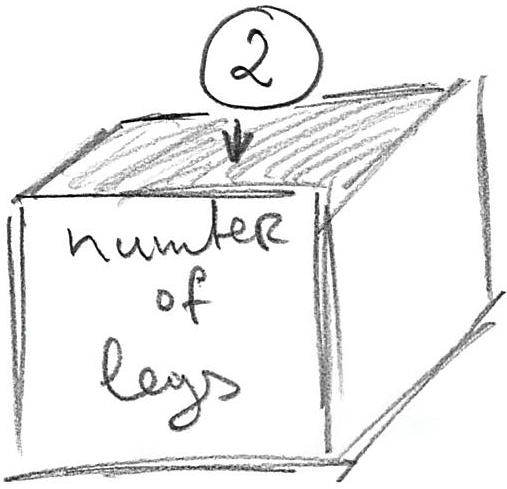
\includegraphics[width=0.5\linewidth]{images/variable-as-box} \end{center}

In Python, you would write

\begin{Shaded}
\begin{Highlighting}[]
\NormalTok{number\_of\_legs }\OperatorTok{=} \DecValTok{2}
\end{Highlighting}
\end{Shaded}

The \textbf{assignment statement} above has very simple structure:

\begin{Shaded}
\begin{Highlighting}[]
\OperatorTok{\textless{}}\NormalTok{variable}\OperatorTok{{-}}\NormalTok{name}\OperatorTok{\textgreater{}} \OperatorTok{=} \OperatorTok{\textless{}}\NormalTok{value}\OperatorTok{\textgreater{}}
\end{Highlighting}
\end{Shaded}

Variable name (name tag on the box) should be meaningful, it can start with letters or \_ and can contain letters, numbers, and \_ symbol but not spaces, tabs, special characters, etc. Python recommends (well, actually, \href{https://www.python.org/dev/peps/pep-0008/}{insists}) that you use \textbf{snake\_case} (all lower-case, underscore for spaces) to format your variable names. The \texttt{\textless{}value\textgreater{}} on the right side is a more complex story, as it can be hard-coded (as in example above), computed using other variables or the same variable, returned by a function, etc.

Using variables means that you can concentrate what corresponding values \textbf{mean} rather than worrying about what these values are. For example, the next time you need to compute something based on number of character's legs (e.g., how many pairs of shoes does a character need), you can compute it based on current value of \texttt{number\_of\_legs} variable rather than assume that it is \texttt{1}.

\begin{Shaded}
\begin{Highlighting}[]
\CommentTok{\# BAD: why 1? Is it because the character has two legs or}
\CommentTok{\# because we issue one pair of shoes per character irrespective of}
\CommentTok{\# their actual number of legs?}
\NormalTok{pairs\_of\_shoes }\OperatorTok{=} \DecValTok{1}

\CommentTok{\# BETTER (but what if our character has only one leg?)}
\NormalTok{pairs\_of\_shoes }\OperatorTok{=}\NormalTok{ number\_of\_legs }\OperatorTok{/} \DecValTok{2}
\end{Highlighting}
\end{Shaded}

Variables also give you flexibility. Their values can change during the program run: player's score is increasing, number of lives decreasing, number of spells it can cast grows or falls depending on their use, etc. Yet, you can always use the value in the variable to perform necessary computations. For example, here is a slightly extended \texttt{number\_of\_shoes} example.

\begin{Shaded}
\begin{Highlighting}[]
\NormalTok{number\_of\_legs }\OperatorTok{=} \DecValTok{2}

\CommentTok{\# ...}
\CommentTok{\# something happens and our character is turned into an octopus}
\NormalTok{number\_of\_legs }\OperatorTok{=} \DecValTok{8}
\CommentTok{\# ...}

\CommentTok{\# the same code still works and we still can compute the correct number of pairs of shoes}
\NormalTok{pairs\_of\_shoes }\OperatorTok{=}\NormalTok{ number\_of\_legs }\OperatorTok{/} \DecValTok{2}
\end{Highlighting}
\end{Shaded}

As noted above, you can think about a variable as a labeled box you can store something in. That means that you can always ``throw away'' the old value and put something new. In case of variables, the ``throwing away'' part happens automatically, as a new value overwrites the old one. Check yourself, what will be final value of the variable in the code below?

\begin{Shaded}
\begin{Highlighting}[]
\NormalTok{number\_of\_legs }\OperatorTok{=} \DecValTok{2}
\NormalTok{number\_of\_legs }\OperatorTok{=} \DecValTok{5}
\NormalTok{number\_of\_legs }\OperatorTok{=} \DecValTok{1}
\NormalTok{number\_of\_legs}
\end{Highlighting}
\end{Shaded}

Do exercise \#1.

As you have already seen, you can \emph{compute} a value instead of specifying it. What would be the answer here?

\begin{Shaded}
\begin{Highlighting}[]
\NormalTok{number\_of\_legs }\OperatorTok{=} \DecValTok{2} \OperatorTok{*} \DecValTok{2}
\NormalTok{number\_of\_legs }\OperatorTok{=} \DecValTok{7} \OperatorTok{{-}} \DecValTok{2}
\NormalTok{number\_of\_legs}
\end{Highlighting}
\end{Shaded}

Do exercise \#2.

\hypertarget{assignments-are-not-equations}{%
\section{Assignments are not equations!}\label{assignments-are-not-equations}}

\textbf{Very important}: although assignments \emph{look} like mathematical equations, they are \textbf{not equations!} They follow a \textbf{very important} rule that you must keep in mind when understanding assignments: the right side of an expression is evaluated \emph{first} until the final value is computed, then and only then that final value is assigned to the variable specified on the left side (put in the box). What this means is that you can use the same variable on \emph{both} sides! Let's take a look at this code:

\begin{Shaded}
\begin{Highlighting}[]
\NormalTok{x }\OperatorTok{=} \DecValTok{2}
\NormalTok{y }\OperatorTok{=} \DecValTok{5}
\NormalTok{x }\OperatorTok{=}\NormalTok{ x }\OperatorTok{+}\NormalTok{ y }\OperatorTok{{-}} \DecValTok{4}
\end{Highlighting}
\end{Shaded}

What happens when computer evaluates the last line? First, it takes \emph{current} values of all variables (\texttt{2} for \texttt{x} and \texttt{5} for \texttt{y}) and puts them into the expression. After that internal step, the expression looks like

\begin{Shaded}
\begin{Highlighting}[]
\NormalTok{x }\OperatorTok{=} \DecValTok{2} \OperatorTok{+} \DecValTok{5} \OperatorTok{{-}} \DecValTok{4}
\end{Highlighting}
\end{Shaded}

Then, it computes the expression on the right side and, \textbf{once the computation is completed}, stores that new value in \texttt{x}

\begin{Shaded}
\begin{Highlighting}[]
\NormalTok{x }\OperatorTok{=} \DecValTok{3}
\end{Highlighting}
\end{Shaded}

Do exercise \#3 to make sure you understand this.

\hypertarget{constants}{%
\section{Constants}\label{constants}}

Although the real power of variables is that you can change their value, you should use them even if the value remains constant throughout the program. There are no true constants in Python, rather an agreement that their names should be all \texttt{UPPER\_CASE}. Accordingly, when you see \texttt{SUCH\_A\_VARIABLE} you know that you should not change its value. Technically, this is just a recommendation, as no one can stop you from modifying value of a \texttt{CONSTANT}. However, much of Python's ease-of-use comes from such agreements (such as a \texttt{snake\_case} convention above). We will encounter more of such agreements later, for example, when learning about objects.

Taking all this into account, if number of legs stays constant throughout the game, you should highlight that constancy and write

\begin{Shaded}
\begin{Highlighting}[]
\NormalTok{NUMBER\_OF\_LEGS }\OperatorTok{=} \DecValTok{2}
\end{Highlighting}
\end{Shaded}

I strongly recommend using constants and avoid hardcoding values. First, if you have several identical values that mean different things (2 legs, 2 eyes, 2 ears, 2 vehicles per character, etc.), seeing a \texttt{2} in the code will not tell you what does this \texttt{2} mean (the legs? the ears? the score multiplier?). You can, of course, figure it out based on the code that uses this number but you could spare yourself that extra effort and use a properly named constant instead. Then, you just read its name and the meaning of the value becomes apparent and it is the meaning not the actual value that you are mostly interested in. Second, if you decide to \emph{change} that value (say, our main character is now a tripod), when using a constant means you have only one place to worry about, the rest of the code stays as is. If you hard-coded that number, you are in for an exciting\footnote{not really} and definitely long search-and-replace throughout the entire code.

Do exercise \#4.

\hypertarget{value-types}{%
\section{Value types}\label{value-types}}

So far, we only used integer numeric values (1, 2, 5, 1000\ldots). Although, Python supports \href{https://docs.python.org/3/library/stdtypes.html}{many different value types}, at first we will concentrate on a small subset of them:

\begin{itemize}
\tightlist
\item
  integer numbers, we already used, e.g.~\texttt{-1}, \texttt{100000}, \texttt{42}.
\item
  float numbers that can take any real value, e.g.~\texttt{42.0}, \texttt{3.14159265359}, \texttt{2.71828}.
\item
  strings that can store text. The text is enclosed between either paired quotes \texttt{"some\ text"} or apostrophes \texttt{\textquotesingle{}some\ text\textquotesingle{}}. This means that you can use quotes or apostrophes inside the string, as long as its is enclosed by the alternative. E.g., \texttt{"students\textquotesingle{}\ homework"} (enclosed in \texttt{"}, apostrophe \texttt{\textquotesingle{}} inside) or \texttt{\textquotesingle{}"All\ generalizations\ are\ false,\ including\ this\ one."\ Mark\ Twain\textquotesingle{}} (quotation enclosed by apostrophes). There is much much more to strings and we will cover that material throughout the course.
\item
  logical / Boolean values that are either \texttt{True} or \texttt{False}.
\end{itemize}

When using a variable it is important that you know what type of value it stores and this is mostly on you. Python will raise an error, if you try doing a computation using incompatible. In some cases, Python will automatically convert values between certain types, e.g.~any integer value is also a real value, so conversion from \texttt{1} to \texttt{1.0} is mostly trivial and automatic. However, in other cases you may need to use explicit conversion. Go to exercise \#5 and try guessing which code will run and which will throw an error due to incompatible types?

\begin{Shaded}
\begin{Highlighting}[]
\DecValTok{5} \OperatorTok{+} \FloatTok{2.0}
\CommentTok{\textquotesingle{}5\textquotesingle{}} \OperatorTok{+} \DecValTok{2}
\CommentTok{\textquotesingle{}5\textquotesingle{}} \OperatorTok{+} \StringTok{\textquotesingle{}2\textquotesingle{}}
\CommentTok{\textquotesingle{}5\textquotesingle{}} \OperatorTok{+} \VariableTok{True}
\DecValTok{5} \OperatorTok{+} \VariableTok{True}
\end{Highlighting}
\end{Shaded}

Do exercise \#5.

Surprised by the last one? This is because internally, \texttt{True} is also \texttt{1} and \texttt{False} is \texttt{0}!

You can explicitly convert from one type to another using special functions. For example, to turn a number or a logical value into a string, you simply write \texttt{str(\textless{}value\textgreater{})}. In examples below, what would be the result?

\begin{Shaded}
\begin{Highlighting}[]
\BuiltInTok{str}\NormalTok{(}\DecValTok{10} \OperatorTok{/} \DecValTok{2}\NormalTok{)}
\BuiltInTok{str}\NormalTok{(}\FloatTok{2.5} \OperatorTok{+} \VariableTok{True}\NormalTok{)}
\BuiltInTok{str}\NormalTok{(}\VariableTok{True}\NormalTok{)}
\end{Highlighting}
\end{Shaded}

Do exercise \#6.

Similarly, you can convert to a logical/Boolean variable using \texttt{bool(\textless{}value\textgreater{})} function. The rules are simple, for numeric values \texttt{0} is \texttt{False}, any other non-zero value is converted to \texttt{True}. For string, an empty string \texttt{\textquotesingle{}\textquotesingle{}} is evaluated to \texttt{False} and non-empty string is converted to \texttt{True}. What would be the output in the examples below?

\begin{Shaded}
\begin{Highlighting}[]
\BuiltInTok{bool}\NormalTok{(}\OperatorTok{{-}}\DecValTok{10}\NormalTok{)}
\BuiltInTok{bool}\NormalTok{(}\FloatTok{0.0}\NormalTok{)}

\NormalTok{secret\_message }\OperatorTok{=} \StringTok{\textquotesingle{}\textquotesingle{}}
\BuiltInTok{bool}\NormalTok{(secret\_message)}

\BuiltInTok{bool}\NormalTok{(}\StringTok{\textquotesingle{}False\textquotesingle{}}\NormalTok{)}
\end{Highlighting}
\end{Shaded}

Do exercise \#7.

Converting to integer or float numbers is trickier. The simplest case is from logical to integer/float, as \texttt{True} gives you \texttt{int(True)} is \texttt{1} and \texttt{float(True)} is \texttt{1.0} and \texttt{False} gives you \texttt{0}/\texttt{0.0}. When converting from float to integer, Python simply drops the fractional part (not rounding!). When converting a string, it must be a valid number of the corresponding type or the error is generated. E.g., you can convert a string like \texttt{"123"} to and integer or a float but this won't work for \texttt{"a123"}. Moreover, you can convert \texttt{"123.4"} to floating-point number but not to an integer, as it has fractional part in it. Given all this, which cells would work and what output would they produce?

\begin{Shaded}
\begin{Highlighting}[]
\BuiltInTok{float}\NormalTok{(}\VariableTok{False}\NormalTok{)}
\BuiltInTok{int}\NormalTok{(}\OperatorTok{{-}}\FloatTok{3.3}\NormalTok{)}
\BuiltInTok{float}\NormalTok{(}\StringTok{"67.8"}\NormalTok{)}
\BuiltInTok{int}\NormalTok{(}\StringTok{"123+3"}\NormalTok{)}
\end{Highlighting}
\end{Shaded}

Do exercise \#8.

\hypertarget{printing-output}{%
\section{Printing output}\label{printing-output}}

To print the value, you need you use \texttt{print()} function (we will talk about functions in general later). In the simplest case, you pass the value and it will be printed out.

\begin{Shaded}
\begin{Highlighting}[]
\BuiltInTok{print}\NormalTok{(}\DecValTok{5}\NormalTok{)}
\CommentTok{\#\textgreater{} 5}
\end{Highlighting}
\end{Shaded}

or

\begin{Shaded}
\begin{Highlighting}[]
\BuiltInTok{print}\NormalTok{(}\StringTok{"five"}\NormalTok{)}
\CommentTok{\#\textgreater{} five}
\end{Highlighting}
\end{Shaded}

Of course, you already know about the variables, so rather than putting a value directly, you can pass a variable instead and its value will be printed out.

\begin{Shaded}
\begin{Highlighting}[]
\NormalTok{number\_of\_pancakes }\OperatorTok{=} \DecValTok{10}
\BuiltInTok{print}\NormalTok{(number\_of\_pancakes)}
\CommentTok{\#\textgreater{} 10}
\end{Highlighting}
\end{Shaded}

or

\begin{Shaded}
\begin{Highlighting}[]
\NormalTok{breakfast }\OperatorTok{=} \StringTok{"pancakes"}
\BuiltInTok{print}\NormalTok{(breakfast)}
\CommentTok{\#\textgreater{} pancakes}
\end{Highlighting}
\end{Shaded}

You can also pass more than one value/variable to the print function and all the values will be printed one after another. For example, if we want to tell the user what did I had for breakfast and just how many of those, we can do

\begin{Shaded}
\begin{Highlighting}[]
\NormalTok{breakfast }\OperatorTok{=} \StringTok{"pancakes"}
\NormalTok{number\_of\_items }\OperatorTok{=} \DecValTok{10}
\BuiltInTok{print}\NormalTok{(breakfast, number\_of\_items)}
\CommentTok{\#\textgreater{} pancakes 10}
\end{Highlighting}
\end{Shaded}

What will be printed by the code below?

\begin{Shaded}
\begin{Highlighting}[]
\NormalTok{dinner }\OperatorTok{=} \StringTok{"stake"}
\NormalTok{count }\OperatorTok{=} \DecValTok{4}
\NormalTok{desert }\OperatorTok{=} \StringTok{"cupcakes"}

\BuiltInTok{print}\NormalTok{(count, dinner, count, desert)}
\end{Highlighting}
\end{Shaded}

Do exercise \#9.

However, you probably would want to be more explicit, when you print out the information. For example, imagine you have these three variables:

\begin{Shaded}
\begin{Highlighting}[]
\NormalTok{meal }\OperatorTok{=} \StringTok{"breakfast"}
\NormalTok{dish }\OperatorTok{=} \StringTok{"pancakes"}
\NormalTok{count }\OperatorTok{=} \DecValTok{10}
\end{Highlighting}
\end{Shaded}

You could, of course do \texttt{print(meal,\ dish,\ count)} but it would be nicer to print ``\emph{I had \textbf{10 pancakes} for \textbf{breakfast}}'', where items in bold would be the inserted variables' values. For this, we need to use string formatting. Please note that the string formatting is not specific to printing, you can create a new string value via formatting and store it in a variable (without printing it out) or print it out (without storing it).

\hypertarget{string-formatting}{%
\section{String formatting}\label{string-formatting}}

A great resource on string formatting in Python is \href{https://pyformat.info/}{pyformat.info}. As Python constantly evolves, it now has more than one way to format strings. Below, I will introduce the ``old'' format that is based on classic string formatting used in \texttt{sprintf} function is C, Matlab, R, and many other programming languages. It is somewhat less flexible than a newer ones but for simple tasks the difference is negligible. Knowing the old format is useful because of its generality. If you want to learn alternatives, read at the link above.

The general call is \texttt{"a\ string\ with\ formatting"\%(tuple\ of\ values\ to\ be\ used\ during\ formatting)}.

In \texttt{"a\ string\ with\ formatting"}, you specify where you want to put the value via \texttt{\%} symbol that is followed by an \emph{optional} formatting info and the \emph{required} symbol that defines the \textbf{type} of the value. The type symbols are

\begin{itemize}
\tightlist
\item
  \texttt{s} for string
\item
  \texttt{d} for an integer
\item
  \texttt{f} for a float value
\item
  \texttt{g} for an ``optimally'' printed float value, so that scientific notation is used for large values (\emph{e.g.}, \texttt{10e5} instead of \texttt{100000}).
\end{itemize}

Here is an example of formatting a string using an integer:

\begin{Shaded}
\begin{Highlighting}[]
\BuiltInTok{print}\NormalTok{(}\StringTok{"I had }\SpecialCharTok{\%d}\StringTok{ pancakes for breakfast"}\OperatorTok{\%}\NormalTok{(}\DecValTok{10}\NormalTok{))}
\CommentTok{\#\textgreater{} I had 10 pancakes for breakfast}
\end{Highlighting}
\end{Shaded}

You are not limited to a single value that you can put into a string. You can specify more locations via \texttt{\%} but you must make sure that you pass the right number of values. Before running it, can you figure out which call will actually work (and what will be the output ) and which will produce an error?

\begin{Shaded}
\begin{Highlighting}[]
\BuiltInTok{print}\NormalTok{(}\StringTok{\textquotesingle{}I had }\SpecialCharTok{\%d}\StringTok{ pancakes and either }\SpecialCharTok{\%d}\StringTok{  or }\SpecialCharTok{\%d}\StringTok{ stakes for dinner\textquotesingle{}}\OperatorTok{\%}\NormalTok{(}\DecValTok{2}\NormalTok{))}
\BuiltInTok{print}\NormalTok{(}\StringTok{\textquotesingle{}I had }\SpecialCharTok{\%d}\StringTok{ pancakes and }\SpecialCharTok{\%d}\StringTok{ stakes for dinner\textquotesingle{}}\OperatorTok{\%}\NormalTok{(}\DecValTok{7}\NormalTok{, }\DecValTok{10}\NormalTok{))}
\BuiltInTok{print}\NormalTok{(}\StringTok{\textquotesingle{}I had }\SpecialCharTok{\%d}\StringTok{ pancakes and }\SpecialCharTok{\%d}\StringTok{ stakes for dinner\textquotesingle{}}\OperatorTok{\%}\NormalTok{(}\DecValTok{1}\NormalTok{, }\DecValTok{7}\NormalTok{, }\DecValTok{10}\NormalTok{))}
\end{Highlighting}
\end{Shaded}

Do exercise \#10.

In case of real values you have two options: \texttt{\%f} and \texttt{\%g}. The latter uses scientific notation (e.g.~\texttt{1e10} for \texttt{10000000000}) to make a representation more compact.

Do exercise \#11 to get a better feeling for the difference.

These is much more to formatting and you can read about it at \href{https://pyformat.info/}{pyformat.info}. However, these basics are sufficient for us to start programming our first game during the next seminar. Don't forget to submit your exercise notebook and see you next time!

  \bibliography{book.bib}

\end{document}
